\documentclass{article}
\usepackage{a0size}
\renewcommand{\tiny}{\fontsize{12}{14}\selectfont}
\renewcommand{\scriptsize}{\fontsize{14.4}{18}\selectfont}   
\renewcommand{\footnotesize}{\fontsize{17.28}{22}\selectfont}
\renewcommand{\small}{\fontsize{20.74}{25}\selectfont}
\renewcommand{\normalsize}{\fontsize{24.88}{30}\selectfont}
\renewcommand{\large}{\fontsize{29.86}{37}\selectfont}
\renewcommand{\Large}{\fontsize{35.83}{45}\selectfont}
\renewcommand{\LARGE}{\fontsize{43}{54}\selectfont}
\renewcommand{\huge}{\fontsize{51.6}{64}\selectfont}
\renewcommand{\Huge}{\fontsize{61.92}{77}\selectfont}
\newcommand{\veryHuge}{\fontsize{74.3}{93}\selectfont}
\newcommand{\VeryHuge}{\fontsize{89.16}{112}\selectfont}
\newcommand{\VERYHuge}{\fontsize{107}{134}\selectfont}


\newcommand{\membersize}{\noindent\fontsize{61.92}{77}\selectfont}
\newcommand{\titlesize}{\noindent\fontsize{72}{80}\selectfont}

% These colours are tried and tested for titles and headers. Don't
% over use color!
\usepackage{color}

\definecolor{college-engineering}{rgb}{0.09,0.25,0.41}
\definecolor{dept-cse}{rgb}{0.26,0.58,0.82}

\renewcommand{\labelitemi}{\textcolor{college-engineering}\textbullet}
\renewcommand{\labelitemii}{\textcolor{college-engineering}{--}}

\setlength{\labelsep}{0.5em}


% see documentation for a0poster class for the size options here
\let\Textsize\normalsize
\def\Head#1{\hrule\smallskip\noindent{\huge\color{college-engineering} \textbf{#1}}\bigskip}
\def\Subhead#1{\noindent{\large\color{college-engineering} #1}\bigskip}


\usepackage{pgfplots}
\pgfplotsset{compat=1.18}
\pgfplotsset{
  xticklabel={$\mathsf{\pgfmathprintnumber{\tick}}$},
  yticklabel={$\mathsf{\pgfmathprintnumber{\tick}}$},
}
\usetikzlibrary{intersections}
\usepackage{lipsum}  

\usepackage[
  paperwidth=90cm,
  paperheight=120cm,
  top=25cm,
  left=9cm,
  right=9cm,
]{geometry}


\usepackage{wallpaper}
\CenterWallPaper{1}{assets/background}

\usepackage{fontspec}
\setmainfont{Arial}

\usepackage[BoldFont, SlantFont]{xeCJK}
\setCJKmainfont{Microsoft JhengHei}

\usepackage[absolute]{textpos}
\TPGrid[80mm,390mm]{15}{12}

\parindent=0pt
\parskip=\baselineskip

\begin{document}
% disable page numbering
\thispagestyle{empty}
\membersize \textbf{第17組:朱劭璿、陳居廷}\hspace{20.5cm}\textbf{指導老師:陳嘉平 教授}
\bigskip

\titlesize \textbf{TSM-Net: 以對抗式時序壓縮自編碼器為基礎的音訊變速演算法 \\
TSM-Net: Temporal Compressing Autoencoder with Adversarial Losses for Time-Scale Modification on Audio Signals}

\begin{textblock}{7.0}(0,0)
\Head{Introduction} \\
\Large
With the advance of technologies and digitalization, we can store and reproduce multimedia content nowadays. An ubiquitous application regarding audio signals called time-scaled modification (TSM) is used in our daily life. It's also known as playback speed control in the video streaming platforms such as YouTube. With the power of artificial intelligence (AI) and modern computation hardware, however, we haven't discovered any method using AI to refine TSM algorithm and leverage the quality of the synthetic audio to the next level.

We proposed a novel TSM approach. While traditional methods use framing technique and spectral approaches use short-time Fourier transform to get high-level units. TSM-Net, our neural-network model encodes the raw audio into a high-level latent representation called Neuralgram. Since the resulting Neuralgram is a two-dimensional image with real values, we apply some existing image resizing techniques on the Neuralgram and decode it using our neural decoder to obtain the time-scaled audio. \\

\medskip
\Head{Related Works} \\
\Large
 Modeling audio is not a trivial task for neural networks. Models that directly generate raw audio waveform are known as vocoder.

\begin{figure}
\begin{center}

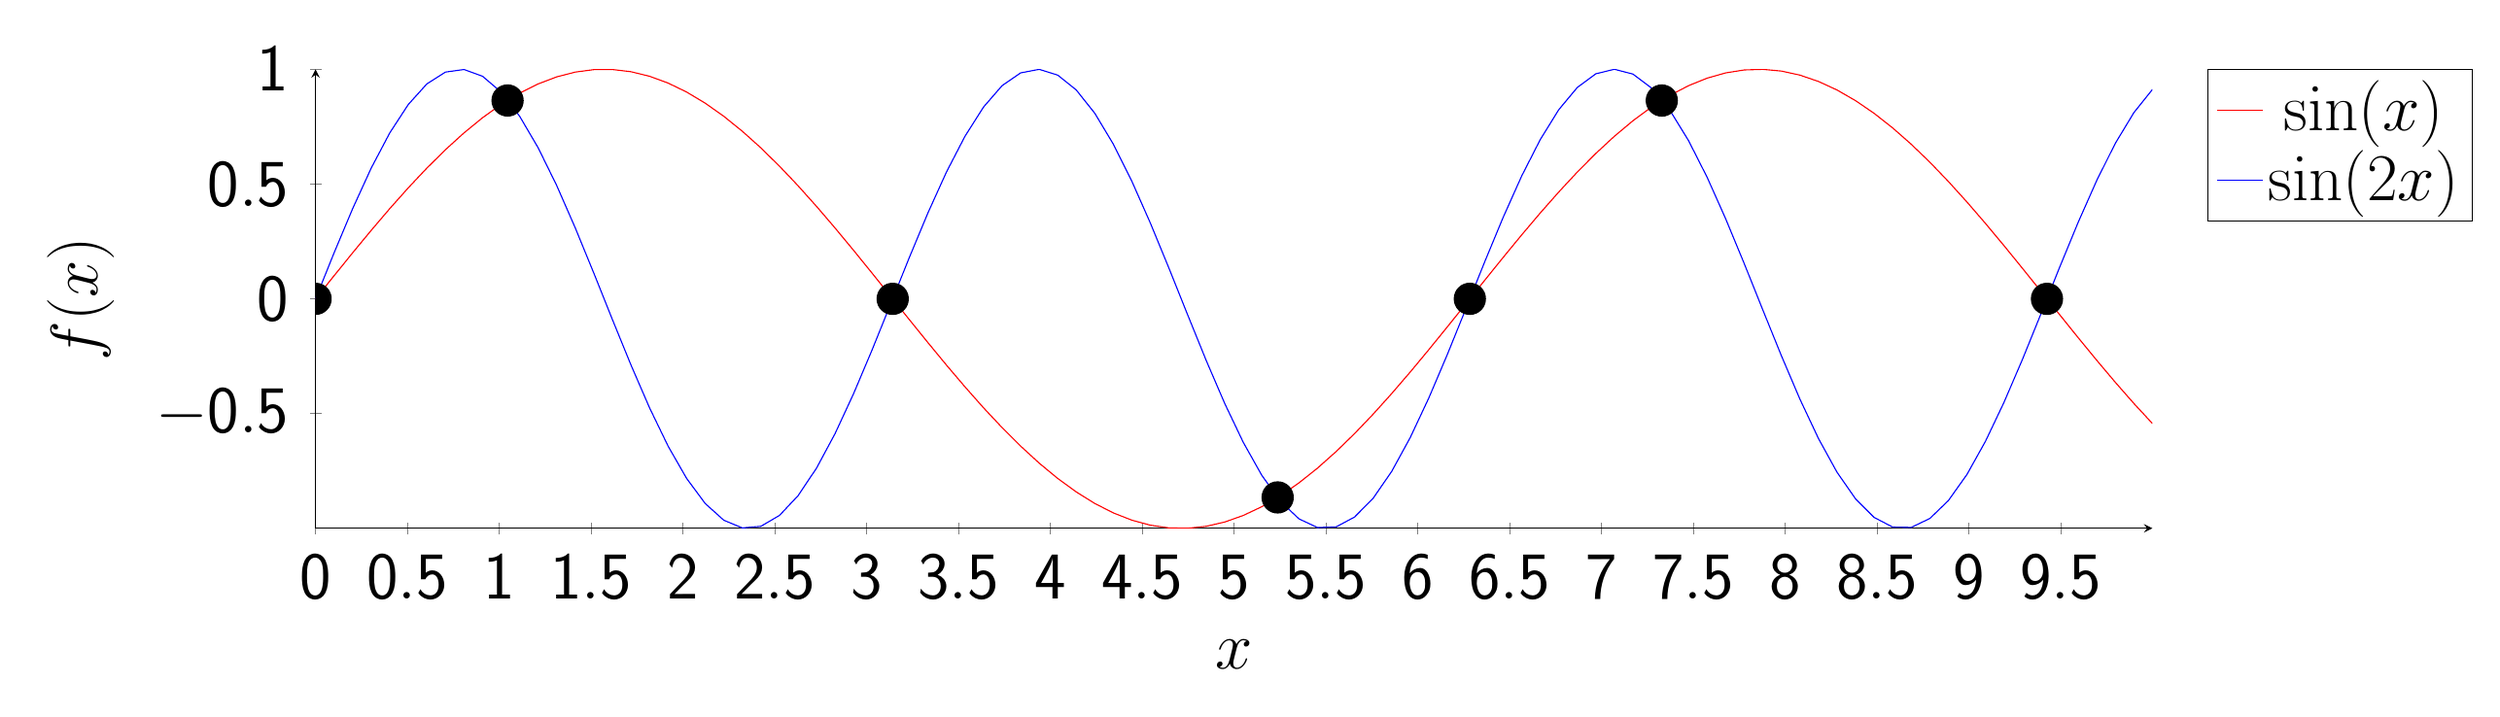
\begin{tikzpicture}
\begin{axis}[
  domain=0:10,
  axis lines = left,
  legend pos=outer north east,
  xlabel=\(x\),
  ylabel={\(f(x)\)},
  width=24cm,
  height=6cm,
  scale only axis,
  legend style={fill=none}
]
\addplot [
  name path=p1,
  samples=100, 
  color=red,
]
{sin(deg(x))};
\addlegendentry{$\sin(x)$}
\addplot [
  name path=p2,
  samples=100, 
  color=blue,
]
{sin(deg(2*x))};
\addlegendentry{$\sin(2x)$}

\fill 
  [name intersections={of=p1 and p2, name=i, total=\t}] 
  [black, opacity=1] 
  \foreach \s in {1,...,\t}{(i-\s) circle (6pt)};

\end{axis}
\end{tikzpicture}

\end{center}
\end{figure}


\medskip
\Head{Methodology} \\
\Large \lipsum[3-3]
\end{textblock}

\begin{textblock}{7.0}(8,0)
\Head{Experiment} \\
\Large \lipsum[4-4]
\large \begin{figure}
\begin{center}
\begin{tabular}{l}
(a)
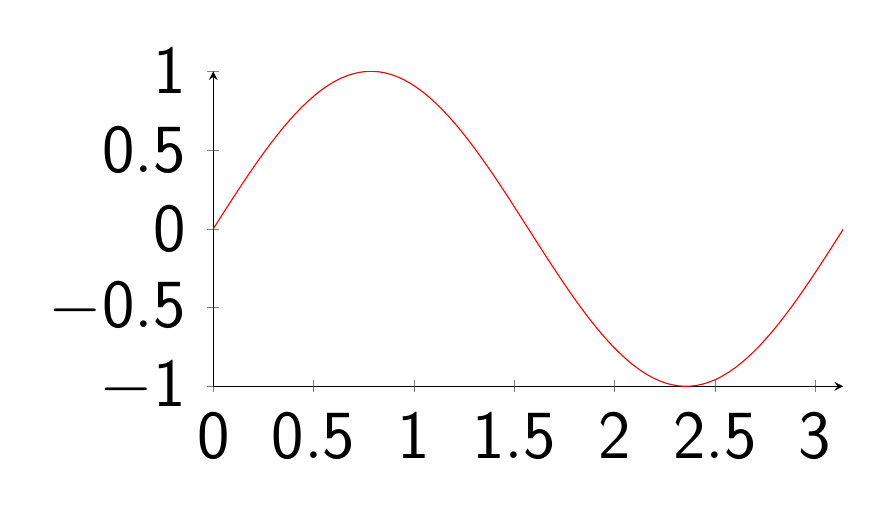
\begin{tikzpicture}
\begin{axis}[
  domain=0:3.14,
  axis lines = left,
  legend pos=outer north east,
  width=8cm,
  height=4cm,
  scale only axis,
]
\addplot [
  samples=100, 
  color=red,
]
{sin(deg(2*x))};

\end{axis}
\end{tikzpicture}

(b)
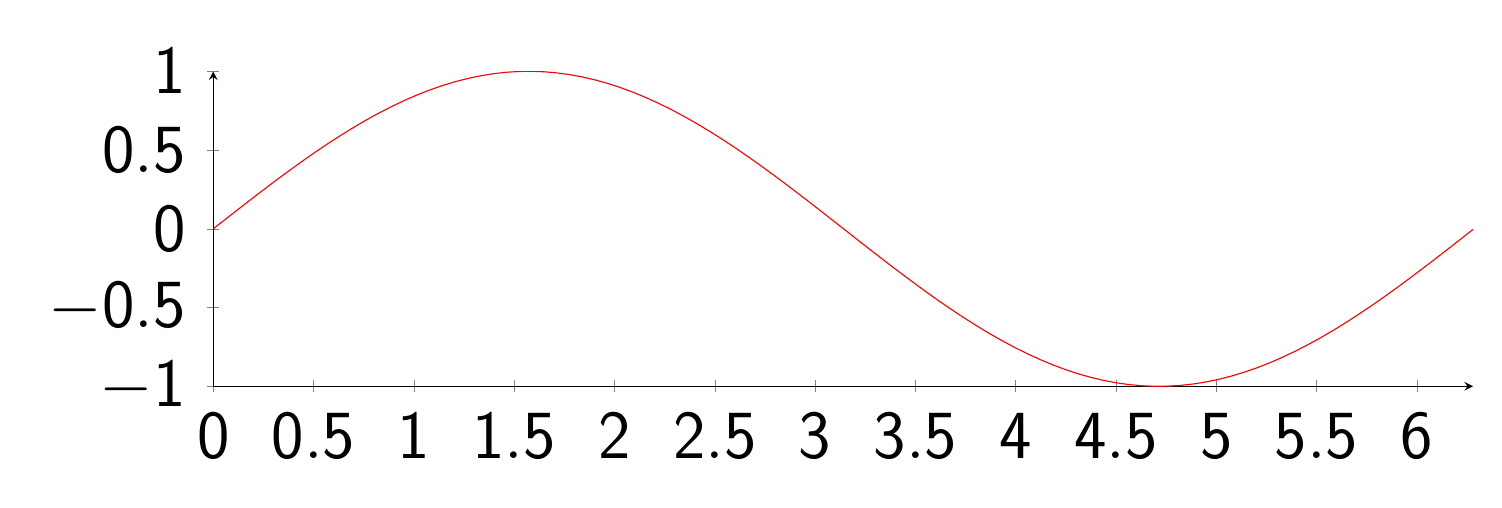
\begin{tikzpicture}
\begin{axis}[
  domain=0:6.28,
  axis lines = left,
  legend pos=outer north east,
  width=16cm,
  height=4cm,
  scale only axis,
]
\addplot [
  samples=100, 
  color=red,
]
{sin(deg(x))};

\end{axis}
\end{tikzpicture} \\

(c)
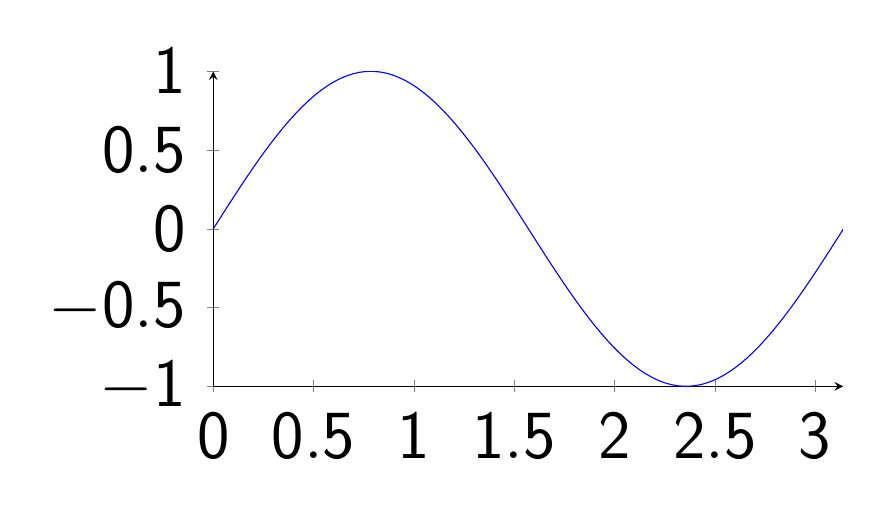
\begin{tikzpicture}
\begin{axis}[
  domain=0:3.14,
  axis lines = left,
  legend pos=outer north east,
  width=8cm,
  height=4cm,
  scale only axis,
]
\addplot [
  samples=100, 
  color=blue,
]
{sin(deg(2*x))};

\end{axis}
\end{tikzpicture}

(d)
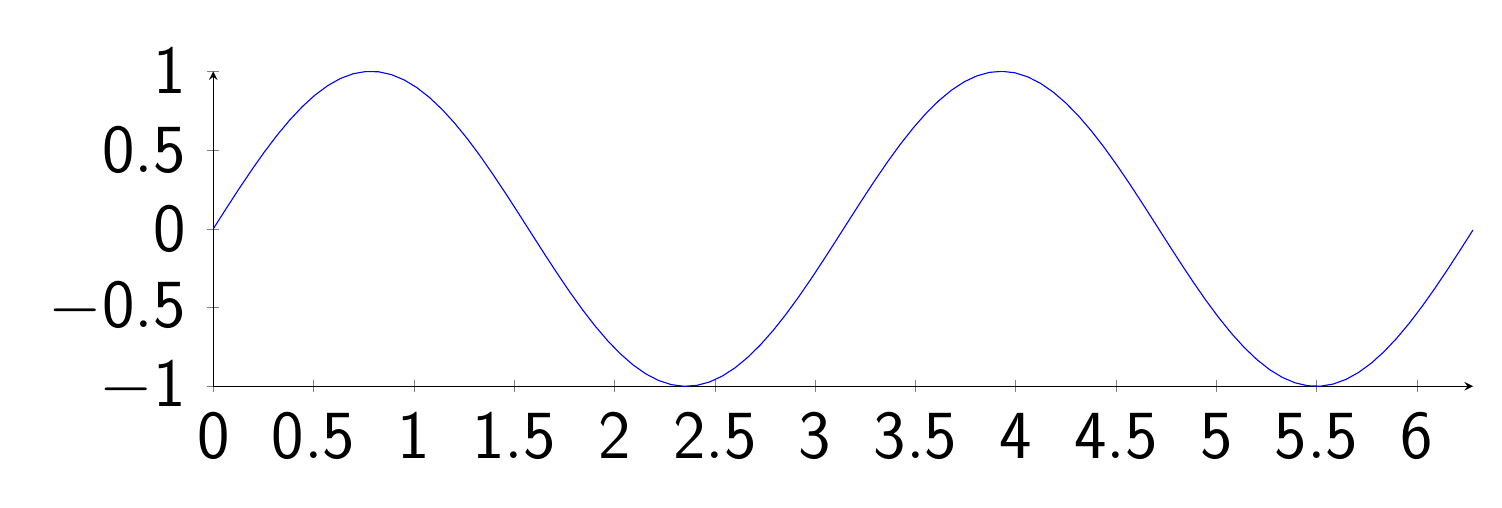
\begin{tikzpicture}
\begin{axis}[
  domain=0:6.28,
  axis lines = left,
  legend pos=outer north east,
  width=16cm,
  height=4cm,
  scale only axis,
]
\addplot [
  samples=100, 
  color=blue,
]
{sin(deg(2*x))};

\end{axis}
\end{tikzpicture}

\end{tabular}
\end{center}
\end{figure}


\medskip
\Head{Conclusion} \\
\Large \lipsum[5-5]
\end{textblock}


\end{document}
